\documentclass[11pt]{article}
\usepackage{graphicx}
\usepackage[a4paper, margin=1in]{geometry}
\usepackage{fontspec}\setmainfont{texgyretermes}[Extension=.otf,UprightFont=*-regular,BoldFont=*-bold,ItalicFont=*-italic,BoldItalicFont=*-bolditalic]
\usepackage{authblk}
\usepackage{url,etoolbox}
\AtBeginEnvironment{thebibliography}{\scriptsize}\let\OLDbib\thebibliography\renewcommand\thebibliography[1]{\OLDbib{#1}\setlength{\parskip}{0pt}\setlength{\itemsep}{0pt}}
\makeatletter\renewcommand\section{\@startsection{section}{1}{0pt}{4pt}{2pt}{\normalsize\bfseries}}\makeatother
\begin{document}
\begin{minipage}{0.2\textwidth}
\includegraphics[width=\textwidth]{ercoftac_logo.png}\end{minipage}\hfill
\begin{minipage}{0.75\textwidth}\fontsize{8}{10}\selectfont\textbf{4th ERCOFTAC Workshop on Machine Learning for Fluid Dynamics, April 2027, Florence, Italy}\end{minipage}
\begin{center}
{\fontsize{15}{18}\selectfont\textbf{Accurate pressure, wrong flow: downstream errors of Darcy neural operators and a loss that removes them}}\\[0.35cm]
\normalsize\textbf{Aryamann Srivastava$^{1}$, Varun Sathaye$^{1}$, Atishay Jain$^{1}$, Vedant S. Tiwari$^{1}$}\\
{\fontsize{9}{10}\selectfont\textit{$^1$Indian Institute of Technology Kanpur, India}}
\end{center}
\noindent
Neural operators for steady Darcy flow, $-\nabla\cdot(\kappa\nabla u)=f$, are ranked by the relative $L^2$ error of the
pressure $u$, usually on PDEBench~\cite{pdebench}. Engineers, however, use the flux $q=-\kappa\nabla u$: effective
permeability, travel times and transport all follow from it. We ask whether pressure accuracy implies flow accuracy, and
answer it against converged references. Building on an independent report that the PDEBench Darcy labels are unconverged
snapshots~\cite{flowguard}, we re-solve the standard $128^2$ split with a self-converged cell-centred finite-volume solver
(0.06\% between $256^2$ and $512^2$); the published labels differ from it by 5.8\% on average, 3.5\% from the boundary
convention and up to 15.5\% from non-convergence on the low-permeability maps usually reported as hardest.

Against converged labels, FNO~\cite{fno} and U-Net~\cite{unet} reach 0.33\% and 0.23\% pressure error but 8.9\% and 5.4\%
error in the conservative face flux, 23 to 27 times more, with up to two thirds of it in the 5\% of cells next to
permeability jumps. To measure what this costs downstream, we solve the pressure-drop problem on the same maps and compute,
from each predicted pressure, the effective permeability $k_{\mathrm{eff}}$ and flux-weighted breakthrough times by
semi-analytical particle tracking (Fig.~\ref{fig:main}). Trained with the usual $L^2$ loss, models with 0.17 to 0.26\%
pressure error have 9 to 15\% $k_{\mathrm{eff}}$ error and 10 to 11\% error in late breakthrough, and the pressure
ranking is reversed: the U-Net is more accurate in pressure but less accurate in $k_{\mathrm{eff}}$. Gradient
supervision with an $H^1$ loss, the common remedy~\cite{sobolevfno}, gives the best pressure (0.13\%) yet still 3.5 to
5.9\% $k_{\mathrm{eff}}$ error. A permeability-weighted face-flux loss, with no change to the architecture, brings both
models to 0.9 to 1.0\% $k_{\mathrm{eff}}$ and 1.7 to 2.3\% late-breakthrough error at the same pressure error. On maps
from an independent generator, where all models are equally accurate in pressure (1.1 to 1.4\%), $k_{\mathrm{eff}}$ errors
are 107 to 665\% with $L^2$, 56 to 66\% with $H^1$ and 10 to 18\% with the face-flux loss. Pressure error is therefore
neither a sufficient nor a monotone proxy for flow accuracy~\cite{betterscores}; we propose flux and downstream
metrics as standard and will release the converged labels, the pressure-drop set and the evaluation code.
\vspace{-4pt}\begin{figure}[h]
\centering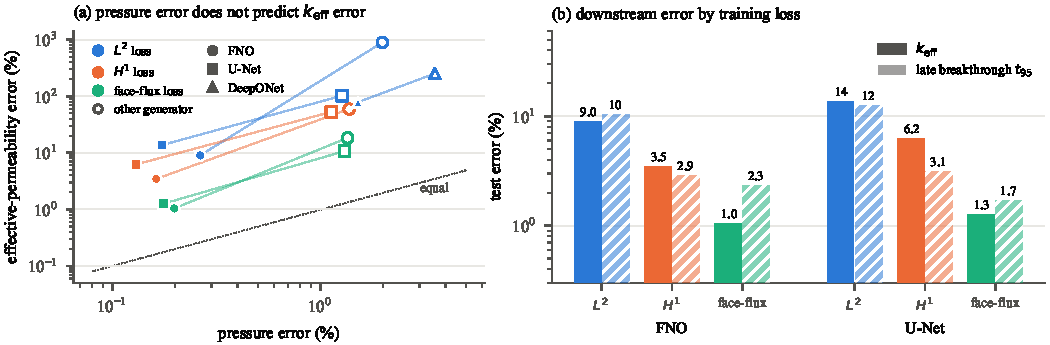
\includegraphics[width=0.9\textwidth]{fig_drop.pdf}
\vspace{-6pt}\caption{\small Pressure-drop problem on the PDEBench maps. (a) Pressure vs $k_{\mathrm{eff}}$ error per model, test split (filled) and independent generator (hollow). (b) Test $k_{\mathrm{eff}}$ and late-breakthrough error by training loss.}
\label{fig:main}
\end{figure}
\vspace{-0.4cm}
\vspace{-6pt}\bibliographystyle{unsrt}\bibliography{refs}
\end{document}
